\begin{name}
	{\tenchude}
	{\tendethi}
	{TRƯỜNG THPT CHUYÊN VĨNH PHÚC - VĨNH PHÚC}
	{\thoigian}
\end{name}

\caulc
% \Opensolutionfile{ans}[Ans/KSCL-THPT-ChuyenVinhPhuc-VinhPhuc-L1-NH24-25-TN]
\Opensolutionfile{ans}[Ans/KSCL-THPT-ChuyenVinhPhuc-VinhPhuc-L1-NH24-25]

%   \Opensolutionfile{ansbook}[Ansbook/KSCL-THPT-ChuyenVinhPhuc-VinhPhuc-L1-NH24-25-TN]%---Nên đặt tên theo bài
  \setcounter{ex}{0}
 %%%==============Cau_EX1==============%%%
\begin{ex}%[Dự án C THPTQG 2025]%[Vương Quốc Phong]%[2D1N1-5]
	\immini[thm]{
	Một doanh nghiệp sản xuất với số lượng là $x$ sản phẩm, $x\in \mathbb{N}$ và thu được lợi nhuận $f(x)$ được biểu thị bởi bảng biến thiên như sau. Hỏi doanh nghiệp sản xuất bao nhiêu sản phẩm trở đi thì lợi nhuận bắt đầu giảm?
	\choice
	{\True $201$}
	{$200$}
	{$101$}
	{$100$}
	}{
\begin{tikzpicture}
			\tkzTabInit[lgt=1.2,espcl=2.5]
			{$x$/.7,$f'(x)$/.7,$f(x)$/1.8}
			{$0$,$200$,$+\infty$}
			\tkzTabLine{ ,+,z,-, }
			\tkzTabVar{-/, +/$100$,-/}
		\end{tikzpicture}}
	\loigiai{
		Dựa vào bảng biến thiên ta thấy lợi nhuận bắt đầu giảm từ sản phẩm $201$.
	}
\end{ex}
%%%==============HetCau_EX1==============%%%

%%%==============Cau_EX2==============%%%
\begin{ex}%[Dự án C THPTQG 2025]%[Vương Quốc Phong]%[2D1N3-1]
	\immini[thm]{
	Cho hàm số $y=f(x)$ có bảng biến thiên trên đoạn $[0;3]$ như sau.
	Giá trị nhỏ nhất của hàm số $y=f(x)$ trên đoạn $[0;3]$ là
	\choice
	{\True $-4$}
	{$1$}
	{$4$}
	{$0$}
	}{
		
\begin{tikzpicture}
			\tkzTabInit[lgt=1.2,espcl=2.5]
			{$x$/.7,$y$/1.8}
			{$0$, $1$, $3$}
			\tkzTabVar{+/$-3$,-/$-4$,+/$0$}
		\end{tikzpicture}
	}
	\loigiai{
		Dựa vào bảng biến thiên ta thấy giá trị nhỏ nhất của hàm số $y=f(x)$ trên đoạn $\left[0;3\right]$ là $-4$.
	}
\end{ex}
%%%==============HetCau_EX2==============%%%

%%%==============Cau_EX3==============%%%
\begin{ex}%[Dự án C THPTQG 2025]%[Vương Quốc Phong]%[1D6H3-2]
	Tập xác định của hàm số $y=\log_{2024} (3-x)$ là
	\choice
	{\True $\mathscr{D} = (-\infty;3)$}
	{$\mathscr{D} = (3;+\infty)$}
	{$\mathscr{D} = (0;+\infty)$}
	{$\mathscr{D} = \mathbb{R}$}
	\loigiai{
		Ta có $3-x > 0 \Leftrightarrow x < 3$. \\
		Vậy $\mathscr{D} = (-\infty;3)$.
	}
\end{ex}
%%%==============HetCau_EX3==============%%%

%%%==============Cau_EX4==============%%%
\begin{ex}%[Dự án C THPTQG 2025]%[Vương Quốc Phong]%[2D1H2-1]
	Cho hàm số $y=f(x)$ xác định trên $\mathbb{R}$ và có đạo hàm $f'(x)=x^{2024} (3-x)$, $\forall x\in \mathbb{R}$. Hàm số đã cho có mấy điểm cực trị?
	\choice
	{$3$}
	{$0$}
	{$2$}
	{\True $1$}
	\loigiai{
	Ta có $f'(x)=x^{2024} (3-x)=0 \Leftrightarrow \hoac{&{x=0} \\ &{x=3}}$, trong đó $x=0$ (nghiệm bội chẵn). \\
	Bảng biến thiên
	\begin{center}
		\begin{tikzpicture}[>=stealth, thick, x=1.2cm, y=1.0cm]
			\def\sohang{5}
			\def\socot{8}
			%ĐN các điểm
			\foreach \x in {1,...,\sohang}
			\foreach \y in {1,...,\socot}
			\path (\y,-\x) coordinate (r{\x}c{\y}) node (r{\x}c{\y}) {};
			%Đường kẻ ngang, dọc
			\draw
			($(r{1}c{1})!.5!(r{2}c{1})+(-.5,0)$)--($(r{1}c{\socot})!.5!(r{2}c{\socot})+(.5,0)$)
			($(r{2}c{1})!.5!(r{3}c{1})+(-.5,0)$)--($(r{2}c{\socot})!.5!(r{3}c{\socot})+(.5,0)$)
			($(r{1}c{1})!.5!(r{1}c{2})+(0,.5)$)--($(r{\sohang}c{1})!.5!(r{\sohang}c{2})+(0,-.5)$)
			;
			%Khung viền
			\draw ($(r{1}c{1})+(-.5,.5)$) rectangle ($(r{\sohang}c{\socot})+(.5,-.5)$);
			%Node các giá trị
			\foreach \diem/\nhan in {
			%Dòng x
			r{1}c{1}/x,r{1}c{2}/\infty,r{1}c{4}/0,r{1}c{6}/3,r{1}c{8}/+\infty,
			%Dòng f'(x)
			r{2}c{1}/f'(x),r{2}c{3}/+,r{2}c{4}/0,r{2}c{5}/+,r{2}c{6}/0,r{2}c{7}/-
			} \path (\diem) node{$\nhan$};
			\path ($(r{3}c{1})!.5!(r{\sohang}c{1})$) node{$f(x)$};
			\foreach \diem/\nhan in {
			%Các dòng của f(x)
			r{3}c{6}/,r{5}c{2}/,r{5}c{8}/
			} \path (\diem) node[shape=rectangle, fill=white, inner sep=2pt] (\diem) {$\nhan$};
			%Vẽ các dấu mũi tên
			\foreach \dau/\cuoi in {r{5}c{2}/r{3}c{6},r{3}c{6}/r{5}c{8}} \draw[->] (\dau)--(\cuoi);
		\end{tikzpicture}
	\end{center}
	Vậy hàm số đã cho có $1$ điểm cực trị.
	}
\end{ex}
%%%==============HetCau_EX4==============%%%

%%%==============Cau_EX5==============%%%
\begin{ex}%[Dự án C THPTQG 2025]%[Vương Quốc Phong]%[1D9H2-5]
	Cho hai biến cố độc lập $A$ và $B$. Biết $P(A)=\dfrac{1}{4}$, $P(A\cup B)=\dfrac{1}{2}$. Tính $P(B)$.
	\choice
	{$\dfrac{3}{4}$}
	{$\dfrac{1}{4}$}
	{$\dfrac{1}{8}$}
	{\True $\dfrac{1}{3}$}
	\loigiai{
		Ta có $P(A\cup B)=P(A)+P(B)-P(AB)=P(A)+P(B)-P(A)\cdot P(B)$ \\
		$\Rightarrow P(B) = \dfrac{P(A \cup B) - P(A)}{1-P(A)} = \dfrac{1}{3}$
	}
\end{ex}
%%%==============HetCau_EX5==============%%%

%%%==============Cau_EX6==============%%%
\begin{ex}%[Dự án C THPTQG 2025]%[Vương Quốc Phong]%[1H8H5-3]
	% \immini{
		Cho hình chóp $S.ABC$ có $SA \perp (ABC)$, $SA=AB=2a$, tam giác $ABC$ vuông tại $B$. Khoảng cách từ $A$ đến mặt phẳng $(SBC)$ bằng
	% }
	% {
	% 	\begin{tikzpicture}[line join = round, line cap = round, thick, font = \small, scale = 0.8]
	% 		\path
	% 		(0:0) coordinate (A)
	% 		+(0:5) coordinate (C)
	% 		+(-50:3) coordinate (B)
	% 		+(90:4) coordinate (S)
	% 		;
	% 		\draw[dashed]
	% 		(A)--(C)
	% 		;
	% 		\draw
	% 		(S)--(A)--(B)--(C)--cycle
	% 		(S)--(B)
	% 		\foreach \x/\y/\z in {S/A/C, S/A/B}{
	% 				pic[draw, angle radius = 8pt]{right angle = \x--\y--\z}
	% 			}
	% 		;
	% 		\foreach \x/\g in {A/180,C/0,B/-90,S/90}
	% 		\fill (\x) circle (1.5pt)
	% 		+(\g:3mm) node {$\x$};
	% 	\end{tikzpicture}
	% }
	\choice
	{$a\sqrt{3}$}
	{\True $a\sqrt{2}$}
	{$a$}
	{$2a$}
	\loigiai{
		\begin{center}
			\begin{tikzpicture}[line join = round, line cap = round, thick, font = \small, scale = 1]
				\path
				(0:0) coordinate (A)
				+(0:5) coordinate (C)
				+(-50:3) coordinate (B)
				+(90:4) coordinate (S)
				($(B)!(A)!(S)$) coordinate (H)
				;
				\draw[dashed]
				(A)--(C)
				;
				\draw
				(S)--(A)--(B)--(C)--cycle
				(S)--(B)
				(A) -- (H)
				;
				\foreach \x/\g in {A/180,C/0,B/-90,S/90, H/45}
				\fill (\x) circle (1.5pt)
				+(\g:3mm) node {$\x$};
			\end{tikzpicture}
		\end{center}
		Ta có $SA \perp (ABC)\Rightarrow SA \perp BC$, $BC \perp AB \Rightarrow BC \perp (SAB) \Rightarrow BC\perp AH$. \\
		Kẻ $AH \perp SB$ và $AH \perp BC \Rightarrow AH \perp (SBC)$, suy ra khoảng cách từ $A$ đến mặt phẳng $(SBC)$ bằng $AH$. \\
		Xét tam giác $SAH$, ta có $\dfrac{1}{AH^2} = \dfrac{1}{SA^2} + \dfrac{1}{AB^2} = \dfrac{1}{2a^2} \Rightarrow AH=a\sqrt{2}$.
	}
\end{ex}
%%%==============HetCau_EX6==============%%%

%%%==============Cau_EX7==============%%%
\begin{ex}%[Dự án C THPTQG 2025]%[Vương Quốc Phong]%[1D1H5-1]
	Biết phương trình $\sin x=m$ có một họ nghiệm là $x=\dfrac{\pi}{5}+k2\pi$, $k\in \mathbb{Z}$. Họ nghiệm còn lại của phương trình đã cho là biểu thức nào sau đây?
	\choice
	{$x=\dfrac{4\pi}{5}+k\pi, k\in \mathbb{Z}$}
	{$x=\dfrac{\pi}{5}+k\pi, k\in \mathbb{Z}$}
	{\True $x=\dfrac{4\pi}{5}+k2\pi, k\in \mathbb{Z}$}
	{$x=-\dfrac{\pi}{5}+k2\pi, k\in \mathbb{Z}$}
	\loigiai{
		Ta có phương trình $\sin x=m$ có một họ nghiệm là $x=\dfrac{\pi}{5}+k\pi, k\in \mathbb{Z}$, họ nghiệm còn lại là $x=\pi-\dfrac{\pi}{5}+k2\pi=\dfrac{4\pi}{5}+k2\pi, k\in \mathbb{Z}$.
	}
\end{ex}
%%%==============HetCau_EX7==============%%%

%%%==============Cau_EX8==============%%%
\begin{ex}%[Dự án C THPTQG 2025]%[Vương Quốc Phong]%[2D1H1-2]
	\immini[thm]{Cho hàm số $y=f(x)$ xác định, có đạo hàm trên $\mathbb{R}$ và $f'(x)$ có đồ thị như hình vẽ. Hàm số $y=f(x)$ đồng biến trên khoảng nào dưới đây?
	\choice
	{$(1;4)$}
	{\True $(-1;1)$}
	{$(1;+\infty)$}
	{$(-\infty;-1)$}
	}{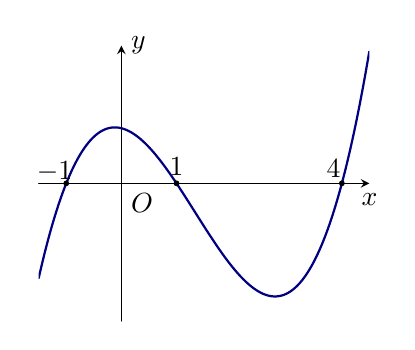
\begin{tikzpicture}[line join = round, line cap = round, >=stealth, scale = .7]
			%Hệ trục Oxy và hàm số cần vẽ
			\def\xmin{-1.5}     \def\xmax{4.5}
			\def\ymin{-2.5}       \def\ymax{2.5}
			\def\f(#1){0.25*(#1)^3-(#1)^2-0.25*(#1)+1}
			%Vẽ hệ trục
			\draw[->] (\xmin,0)--(0,0) node[below right]{$O$}--(\xmax,0) node[below]{$x$};
			\draw[->] (0,\ymin)--(0,\ymax) node[right]{$y$};
			%Vẽ hàm số
			\begin{scope}
				\clip (\xmin,\ymin) rectangle (\xmax,\ymax);
				\draw[smooth, thick, blue!50!black] plot[domain = \xmin:\xmax, samples = 200, variable=\x]({\x},{\f(\x)});
			\end{scope}
			%Vẽ các điểm gióng
			\foreach \x in {}{
					\pgfmathsetmacro\fx{\f(\x)}
					\draw[dashed,thin] (\x,0) |- (0,{\fx});
				}
			\foreach \x/\g in {-1/135, 1/90, 4/120}
			\fill (\x, 0) circle (1.5pt)
			+(\g:3mm) node {$\x$};
		\end{tikzpicture}}
	\loigiai{
		Dựa vào đồ thị ta thấy $f'(x) > 0\Leftrightarrow \hoac{&{-1< x < 1} \\ &{x > 4}}$, suy ra hàm số đồng biến trên $(-1;1)$, $(4;+\infty)$.
	}
\end{ex}
%%%==============HetCau_EX8==============%%%

%%%==============Cau_EX9==============%%%
\begin{ex}%[Dự án C THPTQG 2025]%[Vương Quốc Phong]%[2H2N1-2]
	Cho hình hộp $ABCD.A'B'C'D'$ có đáy $ABCD$ là hình bình hành tâm $O$. Khi đó $2 \cdot \overrightarrow{AO}$ bằng véc-tơ nào sau đây?
	% \begin{center}
	% 	\begin{tikzpicture}[line join = round, line cap = round, thick, font = \small, scale = 1]
	% 		\def \canh{4}
	% 		\path
	% 		(0:0) coordinate (D')
	% 		+(90:\canh) coordinate (D)
	% 		+(0:\canh) coordinate (C')
	% 		+(40:.6*\canh) coordinate (A')
	% 		($(C')+(D)-(D')$) coordinate (C)
	% 		($(D)+(A')-(D')$) coordinate (A)
	% 		($(C')+(A')-(D')$) coordinate (B')
	% 		($(C)+(A)-(D)$) coordinate (B)
	% 		($(A)!.5!(C)$) coordinate (O)
	% 		;
	% 		\draw[dashed]
	% 		(A')--(A) (A')--(B') (A')--(D')
	% 		;
	% 		\draw
	% 		(A)--(B)--(B')--(C')--(D')--(D)--cycle
	% 		(C)--(B) (C)--(D) (C)--(C') (A)--(C)
	% 		;
	% 		\foreach \x/\g in {D'/-90,C'/-90,D/180,A'/135,C/-45,A/90,B'/0,B/90, O/30}
	% 		\fill (\x) circle (1.5pt)
	% 		+(\g:3mm) node {$\x$};
	% 	\end{tikzpicture}
	% \end{center}
	\choice
	{$\overrightarrow{A'C}$}
	{$\overrightarrow{AB}$}
	{$\overrightarrow{AD}$}
	{\True $\overrightarrow{AC}$}
	\loigiai{
		Ta có $2 \cdot \overrightarrow{AO}=\overrightarrow{AC}$.
	}
\end{ex}
%%%==============HetCau_EX9==============%%%

%%%%==============Cau_EX10==============%%%
\begin{ex}%[Dự án C THPTQG 2025]%[Vương Quốc Phong]%[1H8N2-1]
	Trong không gian, qua một điểm $O$ cho trước có bao nhiêu đường thẳng vuông góc với  mặt phẳng $(\alpha)$ cho trước.
	\choice
	{\True $1$}
	{Vô số}
	{$2$}
	{$0$}
	\loigiai{
		Qua một điểm $O$ cho trước có một đường thẳng vuông góc với mặt phẳng $(\alpha)$ cho trước.
	}
\end{ex}
%%%%==============HetCau_EX10==============%%%

%%%%==============Cau_EX11==============%%%
\begin{ex}%[Dự án C THPTQG 2025]%[Vương Quốc Phong]%[2D1N4-1]
	Đường tiệm cận ngang của đồ thị hàm số $y=\dfrac{2x+1}{x+1}$ là
	\choice
	{\True $y=2$}
	{$x=-1$}
	{$y=-1$}
	{$x=2$}
	\loigiai{
		Đường tiệm cận ngang của đồ thị hàm số $y=\dfrac{2x+1}{x+1}$ là $y=2$.
	}
\end{ex}
%%%%==============HetCau_EX11==============%%%

%%%==============Cau_EX12==============%%%
\begin{ex}%[Dự án C THPTQG 2025]%[Vương Quốc Phong]%[1D7H2-1]
	Đạo hàm của hàm số $y=3^x$ là
	\choice
	{\True $y'=3^x \cdot \ln x$}
	{$y'=3^x$}
	{$y'=x\cdot 3^{x-1}$}
	{\True $y'=3^x\cdot \ln 3$}
	\loigiai{
		Đạo hàm của hàm số $y=3^x$ là $y'=3^x \cdot \ln 3$.
	}
\end{ex}
%%%==============HetCau_EX12==============%%%

%  \Closesolutionfile{ans}
%  \Closesolutionfile{ansbook}
 
\cauds
%   \Opensolutionfile{ansbook}[Ansbook/KSCL-THPT-ChuyenVinhPhuc-VinhPhuc-L1-NH24-25-TF]%---Nên đặt tên theo bài
%   \setcounter{ex}{0}
 %%%==============Cau_EX1==============%%%
\begin{ex}%[Dự án C THPTQG 2025]%[Vương Quốc Phong]%[2D1V5-8]
	Theo báo cáo của một cơ sở sản xuất nước tinh khiết, nếu mỗi ngày cơ sở này sản xuất $x$ (m$^3$) nước tinh khiết thì phải chi phí các khoản sau: $3$ triệu đồng chi phí cố định; $0{,}15$ triệu đồng cho mỗi mét khối sản phẩm; $0{,}0003x^2$ chi phí bảo dưỡng máy móc. Biết công suất tối đa mỗi ngày của cơ sở này là $200$ m$^3$. Gọi $C(x)$ là chi phí sản xuất $x$ (m$^3$) sản phẩm mỗi ngày và $\overline{c}(x)$ là chi phí trung bình mỗi mét khối sản phẩm. Khi đó, mệnh đề sau đây đúng hay sai?
	\choiceTF
	{Chi phí sản xuất $100$ m$^3$ nước tinh khiết là $20$ triệu đồng}
	{\True $\overline{c}(x) = 0{,}0003x + 0{,}15 + \dfrac{3}{x}$}
	{\True Chi phí trung bình mỗi mét khối sản phẩm thấp nhất khi sản lượng nước tinh khiết trong ngày là $100$ m$^3$}
	{$C(x) = 0{,}0003x^2 + 0{,}15x + 5$}
	\loigiai{
	Để sản xuất $x$ (m$^3$) nước tinh khiết thì phải chi phí các khoản sau: $3$ triệu đồng chi phí cố định; $0{,}15$ triệu đồng cho mỗi mét khối sản phẩm; $0{,}0003x^2$ chi phí bảo dưỡng máy móc. \\
	Suy ra để sản xuất $1$ (m$^3$) nước tinh khiết thì cần $\dfrac{3}{x}$ triệu đồng chi phí cố định; $0{,}15$ triệu đồng cho mỗi mét khối sản phẩm; $0{,}0003x$ chi phí bảo dưỡng máy móc. \\
	$\Rightarrow \overline{c}(x)=\dfrac{3}{x}+0{,}15+0{,}0003x$. \\
	$\Rightarrow C(x)=\overline{c}(x)\cdot x=3+0{,}15x+0{,}0003x^2$.
	\begin{itemchoice}
		\itemch Chi phí sản xuất $100$ m$^3$ là $C(100)=3+0{,}15 \cdot 100 + 0{,}0003 \cdot 100^2 =21$ (triệu đồng).
		\itemch Ta tìm được $\overline{c}(x)=\dfrac{3}{x}+0{,}15+0{,}0003x$.
		\itemch Hàm chi phí trung bình mỗi mét khối sản phẩm là $\overline{c}(x)=\dfrac{3}{x}+0{,}15+0{,}0003x$, $0< x\le 200$. \\
		Đặt $f(x)=\overline{c}(x)=\dfrac{3}{x}+0{,}15+0{,}0003x$, $0< x\le 200$. \\
		$f'(x)=-\dfrac{3}{x^2}+0{,}0003$. \\
		$f'(x)=0\Rightarrow-3+0{,}0003x^2=0\Rightarrow x=100$. \\
		Bảng biến thiên của hàm $f(x)$.
		\begin{center}
			
\begin{tikzpicture}
				\tkzTabInit[lgt=1.2,espcl=4]
				{$x$/1,$f’(x)$/1,$f(x)$/2}
				{$0$, $100$, $200$}
				\tkzTabLine{ ,-,z,+, }
				\tkzTabVar{+/, -/$0{,}21$, +/}
			\end{tikzpicture}
		\end{center}
		Dựa vào BBT thì chi phí trung bình mỗi mét khối sản phẩm thấp nhất khi sản lượng nước tinh khiết trong ngày là $100$ m$^3$.
		\itemch Ta có: $C(x) = 3 + 0{,}15x+0{,}0003x^2$.
	\end{itemchoice}
	}
\end{ex}
%%%==============HetCau_EX1==============%%%

%%%==============Cau_EX2==============%%%
\begin{ex}%[Dự án C THPTQG 2025]%[Vương Quốc Phong]%[1H8V7-2]
	Cho hình chóp $S.ABC$ có mặt bên $(SAB)$ vuông góc với mặt phẳng đáy và tam giác $SAB$ đều cạnh $2a$. Biết tam giác $ABC$ vuông tại $C$ và cạnh $AC=a\sqrt{3}$. Gọi $H$ là trung điểm $AB$.
	\choiceTF
	{\True Mặt phẳng $(SHC)$ và $(ABC)$ vuông góc với nhau}
	{Thể tích của khối chóp $S.ABC$ bằng $\dfrac{a^3}{6}$}
	{$d(C,(SAB)) = \dfrac{a\sqrt{3}}{3}$}
	{\True $SH \perp (ABC)$}
	\loigiai{
		\begin{center}
			\begin{tikzpicture}[line join = round, line cap = round, thick, font = \small, scale = 1]
				\path
				(0:0) coordinate (B)
				+(0:5) coordinate (C)
				+(-60:3) coordinate (A)
				($(A)!.5!(B)$) coordinate (H)
				++(90:4) coordinate (S)
				;
				\draw[dashed]
				(B)--(C)--(H)
				;
				\draw
				(A)--(B)--(S)--(C)--cycle
				(A)--(S)--(H)
				;
				\foreach \x/\g in {B/180, C/0, S/90, H/210, A/-90}
				\fill (\x) circle (1.5pt)
				+(\g:3mm) node {$\x$};
			\end{tikzpicture}
		\end{center}
		\begin{itemchoice}
			\itemch
			\begin{itemize}
				\item Hình chóp $S.ABC$ có mặt bên $(SAB)$ vuông góc với mặt phẳng đáy và tam giác $SAB$ đều nên $SH \perp AB$, mà $AB$ là giao tuyến của $(SAB)$ và mp đáy nên $SH \perp (ABC)$.
				\item $SH \perp (ABC)$, mà $SH \subset (SHC)$ nên $(SHC)\perp (ABC)$.
			\end{itemize}
			\itemch
			\begin{itemize}
				\item $SH \perp (ABC)$, $SH$ là đường cao của hình chóp, $SH = 2a \dfrac{\sqrt{3}}{2}=a\sqrt{3}$.
				\item Tam giác $ABC$ vuông tại $C$ và cạnh $AC=a\sqrt{3}$, $AB=2a$ nên $BC=\sqrt{(2a)^2-\left(a\sqrt{3} \right)^2}=a$
				\item $S_{ABC}=\dfrac{1}{2} a \cdot a\sqrt{3}=\dfrac{a^2\sqrt{3}}{2}$
				\item $V_{S.ABC}=\dfrac{1}{3} SH \cdot S_{ABC}=\dfrac{1}{3} a\sqrt{3} \cdot \dfrac{a^2\sqrt{3}}{2}=\dfrac{a^3}{2}$
			\end{itemize}
			\itemch $d\left(C, (SAB)\right) = \dfrac{3 \cdot V_{S.ABC}}{_{S_{SAB}}} = \dfrac{3 \cdot a^3}{2 \cdot \dfrac{4a^2\sqrt{3}}{4}}=\dfrac{a\sqrt{3}}{2}$
			\itemch  Theo lập luận trong các câu trên ta có $SH \perp (ABC)$.
		\end{itemchoice}
	}
\end{ex}
%%%==============HetCau_EX2==============%%%

%%%==============Cau_EX3==============%%%
\begin{ex}%[Dự án C THPTQG 2025]%[Vương Quốc Phong]%[2D3H1-3]
	Phòng quản lí đào tạo trường Đại học Kinh tế quốc dân thống kê số giờ làm thêm của một nhóm sinh viên năm thứ tư của trường thu được kết quả như bảng sau:
	\begin{center}
		\begin{tabular}{|c|c|c|c|c|c|}
			\hline
			\thead{\textbf{Số giờ làm thêm (giờ/tuần)}} & $[9; 12)$ & $[12; 15)$ & $[15; 18)$ & $[18; 21)$ & [$21; 24)$ \\
			\hline
			\thead{\textbf{Số sinh viên}}               & $6$       & $12$       & $4$        & $2$        & $1$        \\
			\hline
		\end{tabular}
	\end{center}
	\choiceTF
	{Số giờ làm thêm trung bình của nhóm sinh viên trên trong một tuần là $16{,}5$ giờ}
	{\True Giá trị đại diện của nhóm $[9;12)$ là $10{,}5$}
	{Tứ phân vị thứ ba là $15{,}65$}
	{Nhóm chứa trung vị là $[15;18)$}
	\loigiai{
		\begin{itemchoice}
			\itemch Cỡ mẫu: $n=6+12+4+2+1=25$. \\
			Ta có bảng sau:
			\begin{center}
				\begin{tabular}{|c|c|c|c|c|c|}
					\hline
					\thead{\textbf{Số giờ làm thêm (giờ/tuần)}} & $[9; 12)$ & $[12; 15)$ & $[15; 18)$ & $[18; 21)$ & $[21; 24)$ \\
					\hline
					\thead{\textbf{Giá trị đại diện}}           & $10{,}5$  & $13{,}5$   & $16{,}5$   & $19{,}5$   & $22{,}5$   \\
					\hline
					\thead{\textbf{Số sinh viên}}               & $6$       & $12$       & $4$        & $2$        & $1$        \\
					\hline
				\end{tabular}
			\end{center}
			Số giờ làm thêm trung bình của nhóm sinh viên trên trong một tuần là
			$$\overline{x}=\dfrac{6\cdot 10{,}5+12\cdot 13{,}5+4\cdot 16{,}5+2\cdot 19{,}5+1\cdot 22{,}5}{25}=14{,}1 \text{ (giờ).}$$
			\itemch Giá trị đại diện của nhóm $\left[9;12\right)$ là $10{,}5$.
			\itemch Giả sử $x_1, x_2,\ldots, x_{25}$ số giờ làm thêm của các sinh viên trong mẫu số liệu trên và dãy này đã được sắp xếp theo thứ tự không giảm. \\
			Khi đó, trung vị của mẫu số liệu là $x_{13}$ và tứ phân vị thứ ba là $\dfrac{1}{2} \left(x_{19}+x_{20} \right)$. Vì $x_{19}, x_{20}$ đều thuộc nhóm $\left[15;18\right)$ nên nhóm này chứa tứ phân vị thứ ba. Do đó, tứ phân vị thứ ba là:
			\[Q_3=15+\dfrac{\dfrac{3\cdot 25}{4}-12-6}{4} \cdot \left(18-15\right)=15{,}5625.
			\]
			\itemch  Vì $x_{13}$ thuộc nhóm $\left[12;15\right)$ nên nhóm chứa trung vị là nhóm $\left[12;15\right)$.
		\end{itemchoice}
	}
\end{ex}
%%%==============HetCau_EX3==============%%%

%%%==============Cau_EX4==============%%%
\begin{ex}%[Dự án C THPTQG 2025]%[Vương Quốc Phong]%[2D1V4-3]
	Cho hàm số $f(x)=\dfrac{ax+b}{cx+d}$ với $a,b,c,d\in \mathbb{R}$ và $c \ne 0$ có đồ thị hàm số $y=f'(x)$ nhận đường thẳng $x=-1$ làm tiệm cận đứng như hình vẽ dưới. Biết rằng giá trị lớn nhất của hàm số $y=f(x)$ trên đoạn $\left[-3;-2\right]$ bằng $8$.
	\begin{center}
		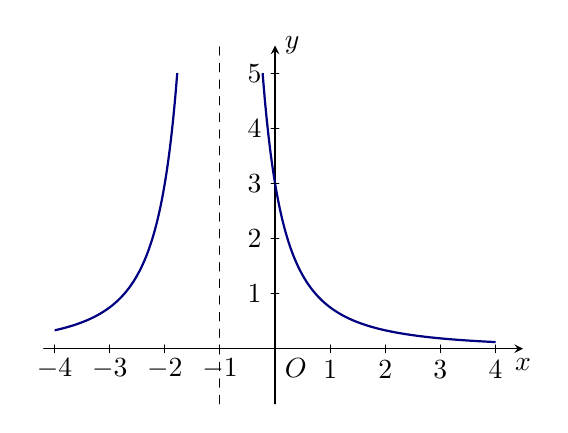
\begin{tikzpicture}[line join = round, line cap = round, >=stealth,  scale = .7]
			%Hệ trục Oxy và hàm số cần vẽ
			\def\xmin{-4}     \def\xmax{4}
			\def\ymin{-1}       \def\ymax{5}
			\def\f(#1){3/((#1)+1)^2}
			%Vẽ hệ trục
			\draw[->] (\xmin-0.2,0)--(0,0) node[below right]{$O$}--(\xmax + 0.5,0) node[below]{$x$};
			\draw[->] (0,\ymin)--(0,\ymax + 0.5) node[right]{$y$};
			%Vẽ hàm số
			\begin{scope}
				\clip (\xmin,\ymin) rectangle (\xmax,\ymax);
				\draw[smooth, thick, blue!50!black] plot[domain = \xmin: -1.4, samples = 200, variable=\x]({\x},{\f(\x)});
				\draw[smooth, thick, blue!50!black] plot[domain = -0.7: \xmax, samples = 200, variable=\x]({\x},{\f(\x)});
			\end{scope}
			\draw[dashed] (-1,-1)--(-1,5.5);
			%Vẽ các điểm gióng
			\foreach \x in {}{
					\pgfmathsetmacro\fx{\f(\x)}
					\draw[dashed,thin] (\x,0) |- (0,{\fx});
				}
			%Vẽ các điểm trên trục Ox
			\foreach \x/\g in {-4/-90,-3/-90,-2/-90,-1/-90,1/-90,2/-90,3/-90,4/-90}
			\draw[thin] (\x,2pt)--(\x,-2pt) + (\g:3mm) node {$\x$};
			%Vẽ các điểm trên trục Oy
			\foreach \y/\g in {1/180,2/180,3/180,4/180,5/180}
			\draw[thin] (2pt,\y)--(-2pt,\y) + (\g:3mm) node {$\y$};
		\end{tikzpicture}
	\end{center}
	\choiceTF
	{\True Giá trị nhỏ nhất của hàm số $y=f(x)$ trên đoạn $\left[2;4\right]$ bằng $4$}
	{$f(-3)=8$}
	{\True Hàm số $y=f(x)$ nghịch biến trên khoảng $(-1;+\infty)$}
	{\True Đồ thị hàm số $y=f'(x)$ nhận đường thẳng $y=0$ làm tiệm cận ngang}
	\loigiai{
		Tập xác định: $\mathscr{D} = \mathbb{R} \setminus \left\{-\dfrac{d}{c} \right\}$. \\
		Ta có $f'(x)=\dfrac{ad-bc}{(cx+d)^2}$.\\
		Đồ thị hàm số $y=f'(x)$ nhận đường thẳng $x=-1$ làm tiệm cận đứng nên $c=d\ne 0$. \\
		Hơn nữa, $f'(x)$ nằm hoàn toàn trên trục hoành nên hàm số $y=f(x)$ đồng biến trên các khoảng xác định và $f'(0)=3$ nên
		\[\heva{&\max\limits_{\left[-3;-2\right]} f(x) = f(-2) = 8 \\ &{\dfrac{ad-bc}{d^2}=3}} \Leftrightarrow \heva{&{\dfrac{2a-b}{d}=8} \\ &{(a-b)d = 3d^2}} \xrightarrow{c=d} \heva{&2a-b=8d \\ & \hoac{&d=0 \text{ (loại)} \\ &a-b=3d}} \Leftrightarrow \heva{&{a=5d} \\&{b=2d}}\]
		Chọn $d=1 \Rightarrow a=5$, $b=2$. \\
		Khi đó $f(x)=\dfrac{5x+2}{x+1} \Rightarrow f'(x)=\dfrac{3}{\left(x+1\right)^2}$.
		\begin{itemchoice}
			\itemch Giá trị nhỏ nhất của hàm số $y=f(x)$ trên đoạn $\left[2;4\right]$ bằng $4$. \\
			Hàm số $y=f(x)$ đồng biến trên $\left[2;4\right]$ nên ${\min \limits_{\left[2;4\right]}} f(x)=f(2)=4$.
			\itemch $f(-3) = \dfrac{5 \cdot (-3) + 2}{-3+2}=\dfrac{13}{2}$.
			\itemch Hàm số $y=f(x)$ đồng biến trên khoảng $\left(-1;+\infty \right)$.
			\itemch Đồ thị hàm số $y=f'(x)$ nhận đường thẳng $y=0$ làm tiệm cận ngang. \\
			Ta có $\lim \limits_{x\to+\infty} f'(x) = \lim \limits_{x\to+\infty} \dfrac{3}{(x+1)^2}=0\Rightarrow y=0$ là TCN của đồ thị hàm số $y=f'(x)$.
		\end{itemchoice}
	}
\end{ex}
%%%==============HetCau_EX4==============%%% \Closesolutionfile{ansbook}
 

\caukq
% \Opensolutionfile{ansbt}[Ansbook/KSCL-THPT-ChuyenVinhPhuc-VinhPhuc-L1-NH24-25-TLN]%---Nên đặt tên theo bài
% \setcounter{ex}{0}
%%%==============Bai_BT1==============%%%
\begin{ex}%[Dự án C THPTQG 2025]%[Vương Quốc Phong]%[2D1V5-8]
	Hai con tàu $A$ và $B$ đang ở cùng một vĩ tuyến và cách nhau $6$ hải lí. Cả hai tàu đồng thời cùng khởi hành. Tàu $A$ chạy về hướng Nam với vận tốc $5$ hải lí/giờ, còn tàu $B$ chạy về vị trí hiện tại của tàu $A$ với vận tốc $7$ hải lí/ giờ. Hỏi sau bao nhiêu giờ thì khoảng cách giữa hai tàu là bé nhất?
	\begin{center}
		\begin{tikzpicture}
			\path
			(0,0) coordinate (A)
			(3,0) coordinate (B1)
			(7,0) coordinate (B)
			(0,-2) coordinate (A1)
			(0,-4) coordinate (A2)
			;
			\draw
			(A2)--(A)node[above]{\Huge{\faShip}}--(B)node[above]{\Huge{\faShip}}
			(A1) -- (B1)
			;
			\draw[-stealth, transform canvas = {xshift = -1 cm}] (A)--(A1);
			\draw[-stealth, yshift = 0.5 cm] (6,0)--(4,0);
			\foreach \x/\g in {A/180,B/-90,A1/180, B1/-90}
			\fill (\x) circle (1.5pt)
			+(\g:3mm) node{$\x$};
		\end{tikzpicture}
	\end{center}
	\shortans{0,57}
	\loigiai{
		Giả sử ban đầu tàu $A$ ở vị trí $A$ và tàu $B$ ở vị trí $B$. Sau khoảng thời gian $t$:
		\begin{itemize}
			\item Tàu $A$ di chuyển được quãng đường $5t$ về phía Nam đến vị trí $A_1$.
			\item Tàu $B$ di chuyển được quãng đường $7t$ đến vị trí $B_1$.
		\end{itemize}
		Khoảng cách từ vị trí $B_1$ đến vị trí $A$ là $6-7t$. \\
		Áp dụng định lý Pytago ta có:  $d=A_1 B_1=f(t)=\sqrt{(6-7t)^2+(5t)^2}=\sqrt{74t^2-84t+36}$. \\
		Để khoảng cách giữa hai tàu nhỏ nhất, thì hàm số $g(t)=74t^2-84t+36$ đạt giá trị nhỏ nhất. \\
		Hàm số $g(t)$ đạt giá trị nhỏ nhất tại $t=\dfrac{-(-84)}{2\cdot 74} = \dfrac{21}{37}$, vậy thời điểm khoảng cách giữa hai tàu bé nhất là khi $t=\dfrac{21}{37} \approx 0{,}57$ (giờ).
	}
\end{ex}
%%%==============HetBai_BT1==============%%%

%%%==============Bai_BT2==============%%%
\begin{ex}%[Dự án C THPTQG 2025]%[Vương Quốc Phong]%[2H2V2-6]
	Có ba lực cùng tác động vào một vật. Hai trong ba lực này hợp với nhau một góc $100^{\circ}$ và có độ lớn lần lượt là $25$ N và $12$ N. Lực thứ ba vuông góc với mặt phẳng tạo bởi hai lực đã cho và có độ lớn $4$ N. Tính độ lớn của hợp lực của ba lực trên (làm tròn đến hàng phần chục).
	\shortans{26,1}
	\loigiai{
		\begin{center}
			\begin{tikzpicture}[line join = round, line cap = round, thick, font = \small, scale = 1]
				\path
				(0:0) coordinate (B)
				+(0:5) coordinate (D)
				+(65:3) coordinate (O)
				($(O)+(D)-(B)$) coordinate (A)
				($(O)+(0,3)$) coordinate (C)
				($(C)+(D)-(O)$) coordinate (E)
				;
				\foreach \x/\y in {O/B, O/A, O/D, O/C}
				\draw[-stealth] (\x)--(\y);
				\draw[dashed]
				(C)--(E)--(D)
				(B)--(D)--(A)
				;
				\foreach \x/\g in {D/-90,C/90,A/90,B/180, O/180, E/90}
				\path (\x)
				+(\g:3mm) node{$\x$};
				\draw[thin] pic[draw, angle radius = 7mm, "$100^{\circ}$", angle eccentricity = 1.5]{ angle = B--O--A};
			\end{tikzpicture}
		\end{center}
		Gọi $\overrightarrow{F_1}$, $\overrightarrow{F_2}$, $\overrightarrow{F_3}$ là ba lực tác động vào vật tại điểm $O$ lần lượt có độ lớn $25$ N, $12$ N, $4$ N. \\
		Vẽ $\overrightarrow{OA}=\overrightarrow{F_1}$, $ \overrightarrow{OB}=\overrightarrow{F_2}$, $ \overrightarrow{OC}=\overrightarrow{F_3}$, dựng hình bình hành $OADB$ và $ODEC$. \\
		Khi đó hợp lực tác động vào vật là: $\overrightarrow{F}=\overrightarrow{OA}+\overrightarrow{OB}+\overrightarrow{OC}=\overrightarrow{OD}+\overrightarrow{OC}=\overrightarrow{OE}$. \\
		Áp dụng định lý cô sin trong tam giác $OBD$, ta có:
		\[OD^2 = OB^2 + BD^2 - 2OB \cdot BD \cos \widehat{OBD}=12^2+25^2-2 \cdot 12 \cdot 25 \cdot \cos 80^{\circ}=769-600 \cdot \cos 80^\circ
		\]
		Vì $OC \perp (OADB)$ nên $OC\perp OD$, suy ra $ODEC$ là hình chữ nhật. Do đó tam giác $ODE$ vuông tại $D$. Ta có $OE=\sqrt{OD^2+ED^2} \approx 26{,}1$
	}
\end{ex}
%%%==============HetBai_BT2==============%%%

%%%==============Bai_BT3==============%%%
\begin{ex}%[Dự án C THPTQG 2025]%[Vương Quốc Phong]%[1D6V4-6]
	Dân số trung bình sơ bộ năm $2021$ của tỉnh Vĩnh Phúc là $1.191.782$ người, tăng $1{,}75\%$ so với năm $2020$. Hỏi với tốc độ tăng dân số được duy trì mức $1{,}75\%$ một năm thì đến năm bao nhiêu dân số tỉnh Vĩnh Phúc lần đầu vượt $1.880.000$ người.
	\shortans{2048}
	\loigiai{
	Áp dụng công thức tăng trưởng dân số thì dân số của tỉnh Vĩnh Phúc sau $n$ năm (tính từ năm $2021$) được tính theo công thức:
	\[S_n=S_0 \cdot e^{rn}=1191782 \cdot \mathrm{e}^{0{,}0175n}
	\]
	Để dân số tỉnh Vĩnh Phúc sau $n$ năm vượt $1.880.000$ người điều kiện là:
	\begin{eqnarray*}
		&& S_n > 1880000 \\ &\Leftrightarrow& 1191782 \cdot \mathrm{e}^{0{,}0175n} > 1880000 \\ &\Leftrightarrow& \mathrm{e}^{0{,}0175n} > \dfrac{1880000}{1191782} \Leftrightarrow 0{,}0175n > \ln \left(\dfrac{1880000}{1191782} \right) \\ &\Leftrightarrow& n > \dfrac{\ln \left(\dfrac{1880000}{1191782} \right)}{0{,}0175} \approx 26{,}047
	\end{eqnarray*}
	Mà $n \in \mathbb{N}$ nên $n\ge 27$.
	Vậy năm $2048$ là năm đầu tiên dân số tỉnh Vĩnh Phúc vượt $1.880.000$ người.
	}
\end{ex}
%%%==============HetBai_BT3==============%%%

%%%==============Bai_BT4==============%%%
\begin{ex}%[Dự án C THPTQG 2025]%[Vương Quốc Phong]%[0D0C2-9]
	Hai bạn Nga và Nhung chơi trò tung xúc xắc. Mỗi bạn tung $1$ con xúc xắc $3$ lần, ai có tổng số chấm $3$ lần gieo lớn hơn thì thắng. Nga chơi trước và được $14$ chấm. Khi đó, xác suất để Nhung thắng Nga là $\dfrac{a}{b}$ (với $a,b$ là số nguyên dương và $\dfrac{a}{b}$ là phân số tối giản). Tính $a+b$. \\
	\shortans{59}
	\loigiai{
		Gọi $A$ là biến cố: \lq\lq Nhung thắng Nga sau ba lần tung\rq\rq.\\
		Khi đó $P(A)$ là xác suất tổng số chấm Nga tung được sau ba lần tung lớn hơn $14$. \\
		Ta có: $\Omega=\left\{(a_1, a_2, a_3)|a_i \in \{1,2,\ldots, 6\}, i=\overline{1,3}\right\}\Rightarrow n(\Omega)=6^3=216$
		\[A=\left\{(a_1, a_2, a_3)|a_1+a_2+a_3 \ge 15, a_i \in \{1,2,\ldots, 6\}, i=\overline{1,3}\right\}
		\]
		Để đếm số phần tử của $A$, ta chia thành các trường hợp:
		\begin{itemize}
			\item Trường hợp 1: $a_1+a_2+a_3=15$, gồm bộ $(5,5,5)$ và các bộ là hoán vị của $(4;5;6)$ và $(3;6;6)$. Trường hợp này có $1+6+3=10$ (bộ)
			\item  Trường hợp 2: $a_1+a_2+a_3=16$, gồm các hoán vị của $(5,5,6)$ và $(4,6,6)$. Trường hợp này có $3+3=6$ (bộ)
			\item  Trường hợp 3: $a_1+a_2+a_3=17$, gồm các hoán vị của $(5,6,6)$. Trường hợp này có $3$ (bộ).
			\item Trường hợp 4: $a_1+a_2+a_3=18$, gồm $(6,6,6)$. Trường hợp này có $1$ (bộ).
		\end{itemize}
		Vậy $n(A)=20$. \\
		Xác suất cần tìm: $P(A)=\dfrac{n(A)}{n(\Omega)}=\dfrac{20}{216}=\dfrac{5}{54} \Rightarrow a+b=59$.
	}
\end{ex}
%%%==============HetBai_BT4==============%%%

%%%==============Bai_BT5==============%%%
\begin{ex}%[Dự án C THPTQG 2025]%[Vương Quốc Phong]%[1H8V5-3]
	Cho hình chóp $S.ABC$ có đáy $ABC$ là tam giác đều cạnh bằng $2$, $SA$ vuông góc với mặt phẳng $(ABC)$; Góc giữa đường thẳng $SB$ và mặt phẳng $(ABC)$ bằng $60^\circ$. Gọi $M$ là trung điểm của cạnh $AB$. Tính khoảng cách từ điểm $B$ đến mặt phẳng $(SCM)$, kết quả làm tròn đến phần trăm.
	\shortans{0,96}
	\loigiai{
		\begin{center}
			\begin{tikzpicture}[line join = round, line cap = round, thick, font = \small, scale = 1]
				\path
				(0:0) coordinate (A)
				+(0:5) coordinate (C)
				+(-50:3) coordinate (B)
				+(90:4) coordinate (S)
				($(A)!.5!(B)$) coordinate (M)
				($(S)!0.65!(M)$) coordinate (H)
				;
				\draw[dashed]
				(A)--(C)--(M)
				;
				\draw
				(S)--(A)--(B)--(C)--cycle
				(S)--(B) (S)--(M) (A)--(H)
				\foreach \x/\y/\z in {C/M/B, A/H/M}{
						pic[draw, angle radius = 6pt]{right angle = \x--\y--\z}
					}
				;
				\foreach \x/\g in {B/-90, C/0, A/180, S/90, M/180, H/145}
				\fill (\x) circle (1.5pt)
				+(\g:3mm) node {$\x$};
			\end{tikzpicture}
		\end{center}
		Vì $AB$ là hình chiếu của $SB$ trên mặt phẳng $(ABC)$, nên góc giữa đường thẳng $SB$ và mặt phẳng $(ABC)$ bằng góc $\widehat{SBA}=60^\circ \Rightarrow SA = AB \cdot \tan 60^\circ=2\sqrt{3}$. \\
		Do $M=AB\cap (SCM)$, $M$ là trung điểm của $AB \Rightarrow d(A,(SCM))= d(B,(SCM))$. \\
		Vì $\heva{&{CM\perp AB} \\ &{CM\perp SA}} \Rightarrow CM\perp (SAB)$. \\
		Mặt khác $CM \subset (SCM)\Rightarrow (SCM)\perp (SAB)$, và $(SCM)\cap (SAB)=SM$, nên kẻ $AH\perp SM$ tại $H$ \\
		$\Rightarrow AH\perp (SMB)\Rightarrow AH = d(A,(SMC)) = d(B,(SMC))$. \\
		Xét tam giác $SAM$ vuông tại $A$, ta có $\dfrac{1}{AH^2}=\dfrac{1}{SA^2}+\dfrac{1}{AM^2}=\dfrac{1}{(2\sqrt{3})^2}+\dfrac{1}{1^2}=\dfrac{13}{12} \Rightarrow AH^2=\dfrac{12}{13} \Rightarrow AH=\sqrt{\dfrac{12}{13}} \approx 0{,}96$. \\
		Vậy khoảng cách từ điểm $B$ đến mặt phẳng $(BCM)$ bằng $0{,}96$
	}
\end{ex}
%%%==============HetBai_BT5==============%%%

%%%==============Bai_BT6==============%%%
\begin{ex}%[Dự án C THPTQG 2025]%[Vương Quốc Phong]%[2D1C5-4]
	Cho hàm số $f(x)=x(x-3)^2$. Tính số nghiệm thực của phương trình $\underbrace{f(f \cdots f(x))}_{8 \text{ lần } f}=0$.
	\shortans{3281}
	\loigiai{
		Ta có $f(x)=x(x-3)^2=x^3-6x^2+9x$. \\
		Suy ra $f'(x)=3x^2-12x+9$. \\
		$f'(x)=0\Leftrightarrow \hoac{&{x=0} \\ &{x=3}}$ \\
		Bảng biến thiên
		\begin{center}
			\begin{tikzpicture}[font=\normalsize,t style/.style={style=solid}]
				%dòng khai báo
				\tkzTabInit[lgt=1.2,espcl=1.75,deltacl=0.5]
				{$x$/0.75,$f'(x)$/0.75, $f(x)$/2}
				{$-\infty$, $0$, $1$, $3$, $4$, $+\infty$}
				%dòng xét dấu của đạo hàm
				\tkzTabLine{,, ,+, 0,-, 0,+ , ,,} % z, t, d, h (h: tô miền);
				%Khai báo vị trị các điểm của dòng f(x)
				\path (N13) node[above] (A1){$ -\infty $}
				($(N32)!0.2!(N33)$) node[below] (A2){$ 4 $}
				($(N42)!0.6!(N43)$) node[left] (A3){$ 0 $}
				(N62) node[below] (A4){$ +\infty $}
				($(N22)!0.6!(N23)$) coordinate (B) node[below] {$0$}
				($(N52)!0.3!(N53)$) coordinate (C) node[below] {$4$}
				;
				\draw[dashed]
				(N21)--(B)--(A3)
				(N51)--(C)--(A2)
				;
				\foreach \x/\y in {A1/A2,A2/A3,A3/A4}{
						\draw[-stealth] (\x)--(\y);
					}
			\end{tikzpicture}
		\end{center}
		Ta có
		$f(x)=0$ có $2$ nghiệm. \\
		$f(x)=3$ có $3$ nghiệm. \\
		$\Rightarrow f\left(f(x)\right)=0\Leftrightarrow \hoac{&{f(x)=0} \\ &{f(x)=3}}$ có $2+3^1$ nghiệm. \\
		$f\left(f\left(f(x)\right)\right)=0\Leftrightarrow \hoac{&{f\left(f(x)\right)=0} \\ &{f\left(f(x)\right)=3}}$ có $2+3^1+3^2$ nghiệm. \\
		$\dots$
		$f\left(f\left(\cdots f(x)\right)\right)=0$ có $2+3^1+3^2+\cdots + 3^7 = 3281$ nghiệm.
	}
\end{ex}
%%%==============HetBai_BT6==============%%%

 \Closesolutionfile{ans}
\inputansbox{6,4,3}{ans/KSCL-THPT-ChuyenVinhPhuc-VinhPhuc-L1-NH24-25}%---Nên đặt tên theo bài
 